\documentclass{beamer}
\usetheme{Boadilla}
\usepackage{tikz}
\usepackage{graphicx}
\usepackage{amsmath}
\usetikzlibrary{shapes.geometric,arrows, positioning, fit}
\tikzstyle{computing} = [draw, rectangle, fill=white!50, rounded corners, node distance=2cm,
                    minimum height=3em]

\tikzstyle{io} = [rectangle, draw, trapezium right angle=110, rounded corners,
                  fill=red!20, node distance=1.9cm, minimum height=2.9em]

\tikzstyle{calculate} = [diamond, draw, trapezium right angle=110, rounded corners,
                  fill=green!20, node distance=1.9cm, minimum height=2.9em]

\tikzstyle{hardware} = [rectangle, draw, trapezium right angle=110, rounded corners,
                  fill=blue!20, node distance=1.9cm, minimum height=2.9em]

\tikzstyle{external} = [rectangle, draw, trapezium right angle=110, rounded corners,
                  fill=gray!20, node distance=1.9cm, minimum height=2.9em]
\tikzstyle{line} = [draw, -latex']

\tikzstyle{function} = [rectangle, draw, fill=green!20, node distance=1.9cm, minimum height=2.9em]
\tikzstyle{ros} = [circle, draw,
                  fill=gray!20, node distance=1.9cm, minimum height=2.9em]

                  \tikzstyle{Process} = [rectangle, draw]

                  \tikzstyle{Start} = [draw, rectangle, rounded corners] 
                  
                  \tikzstyle{Data} = [draw,trapezium,trapezium left angle=70,trapezium right angle=-70]





\title{Midterm Presentation}
\subtitle{AIMBOT}
\author{Martin Blaszczyk \\ Edward Källstedt}
\institute{Luleå University of Technology}
\date{\today}



\begin{document}
\begin{frame}
    \titlepage
\end{frame}

\begin{frame}
    \frametitle{Overview}
    \tableofcontents
\end{frame}


%%%%%%%%%%%% Add new frames below this line %%%%%%%%%
\section{Project structure}
\begin{frame}
    \subsection{Team}
    \frametitle{Group members }
    \begin{itemize}
        \item Y-students
        \begin{itemize}
            \item Martin Blaszczyk - Project leader and object detection
            \item Edward Cedergård -Arm and gripping tool
            \item Niklad Dahlqvist -  Arm and gripping tool
            \item Måns Norell - Movable base
        \end{itemize}
        \item D-students
        \begin{itemize}
            \item Edward Källstedt - Object detection
            \item Albin Martinsson - Arrowhead and Git
        \end{itemize}  
    \end{itemize}
\end{frame}
\begin{frame}
    \subsection{Time plan}
    \frametitle{Overall timetable}
    \begin{table}
        \begin{tabular}{| l | c | c | c | c }
            
            Sep & Oct & Nov & Dec \\
            \hline \hline
            Concept generation & Evaluation & Evaluation &  \\ 
            \hline
            Theory & Prototyping & Evaluation & Finishing up \\
            \hline
            Simulation & Evaluation & Evaluation & \\
            \hline
            Prototyping & Final Design & Evaluation &  \\
            \hline
 
        \end{tabular}
    \end{table}    
\end{frame}


\begin{frame}
    \frametitle{Time plan for September}
    \begin{table}
        \begin{tabular}{l | c | c | c | c }
        Subproject & Week 1 & Week 2 & Week 3 & Week 4 \\
        \hline \hline
            Arrowhead & Reading& Setup & API & Prototyping\\
            Movable base & Reading& Modeling & Simulation & Implementation\\
            Arm and grip  & Reading & Kinematics & Simulation& Prototyping\\
            Object detection & Reading & Testing & Prototyping & Evaluation\\
        \end{tabular}
    \end{table}
\end{frame}

\section{Engineering challenge}
\subsection{Concept}

\subsection{Mechanical structure}
The design of the robot is influenced by the LEGO\textregistered Mindstorms\textregistered EV3 set. While the original set has a movable base without a manipulator arm. It also does not incorporate the Dynamixel AX-12A Smart Servos used in the final design so the decision to redesign the robot with inspiration from the LEGO\textregistered EV3 design was made. By developing and designing a new platform it gave the possibility to adapt the dimensions and fastenings. It also gave experience in manufacturing methods such as 3D-printing and Laser cutting. The final design is shown in Fig. \ref{fig:concept_rendering}
Consisting of seven Dynamixel\textregistered AX-12A Smart Servos for actuation, two on the base for locomotion and four on the arm and one for the gripping tool the robot has seven degrees of freedom. The main advantage of using the AX-12As is the possibility of connecting them in series which enables pararell control of all the joints. Additionaly with the built in sensors the motors return feedback of the joint angles, angular speed, current draw, teperature to name a few.  

\begin{figure}
    \centering
    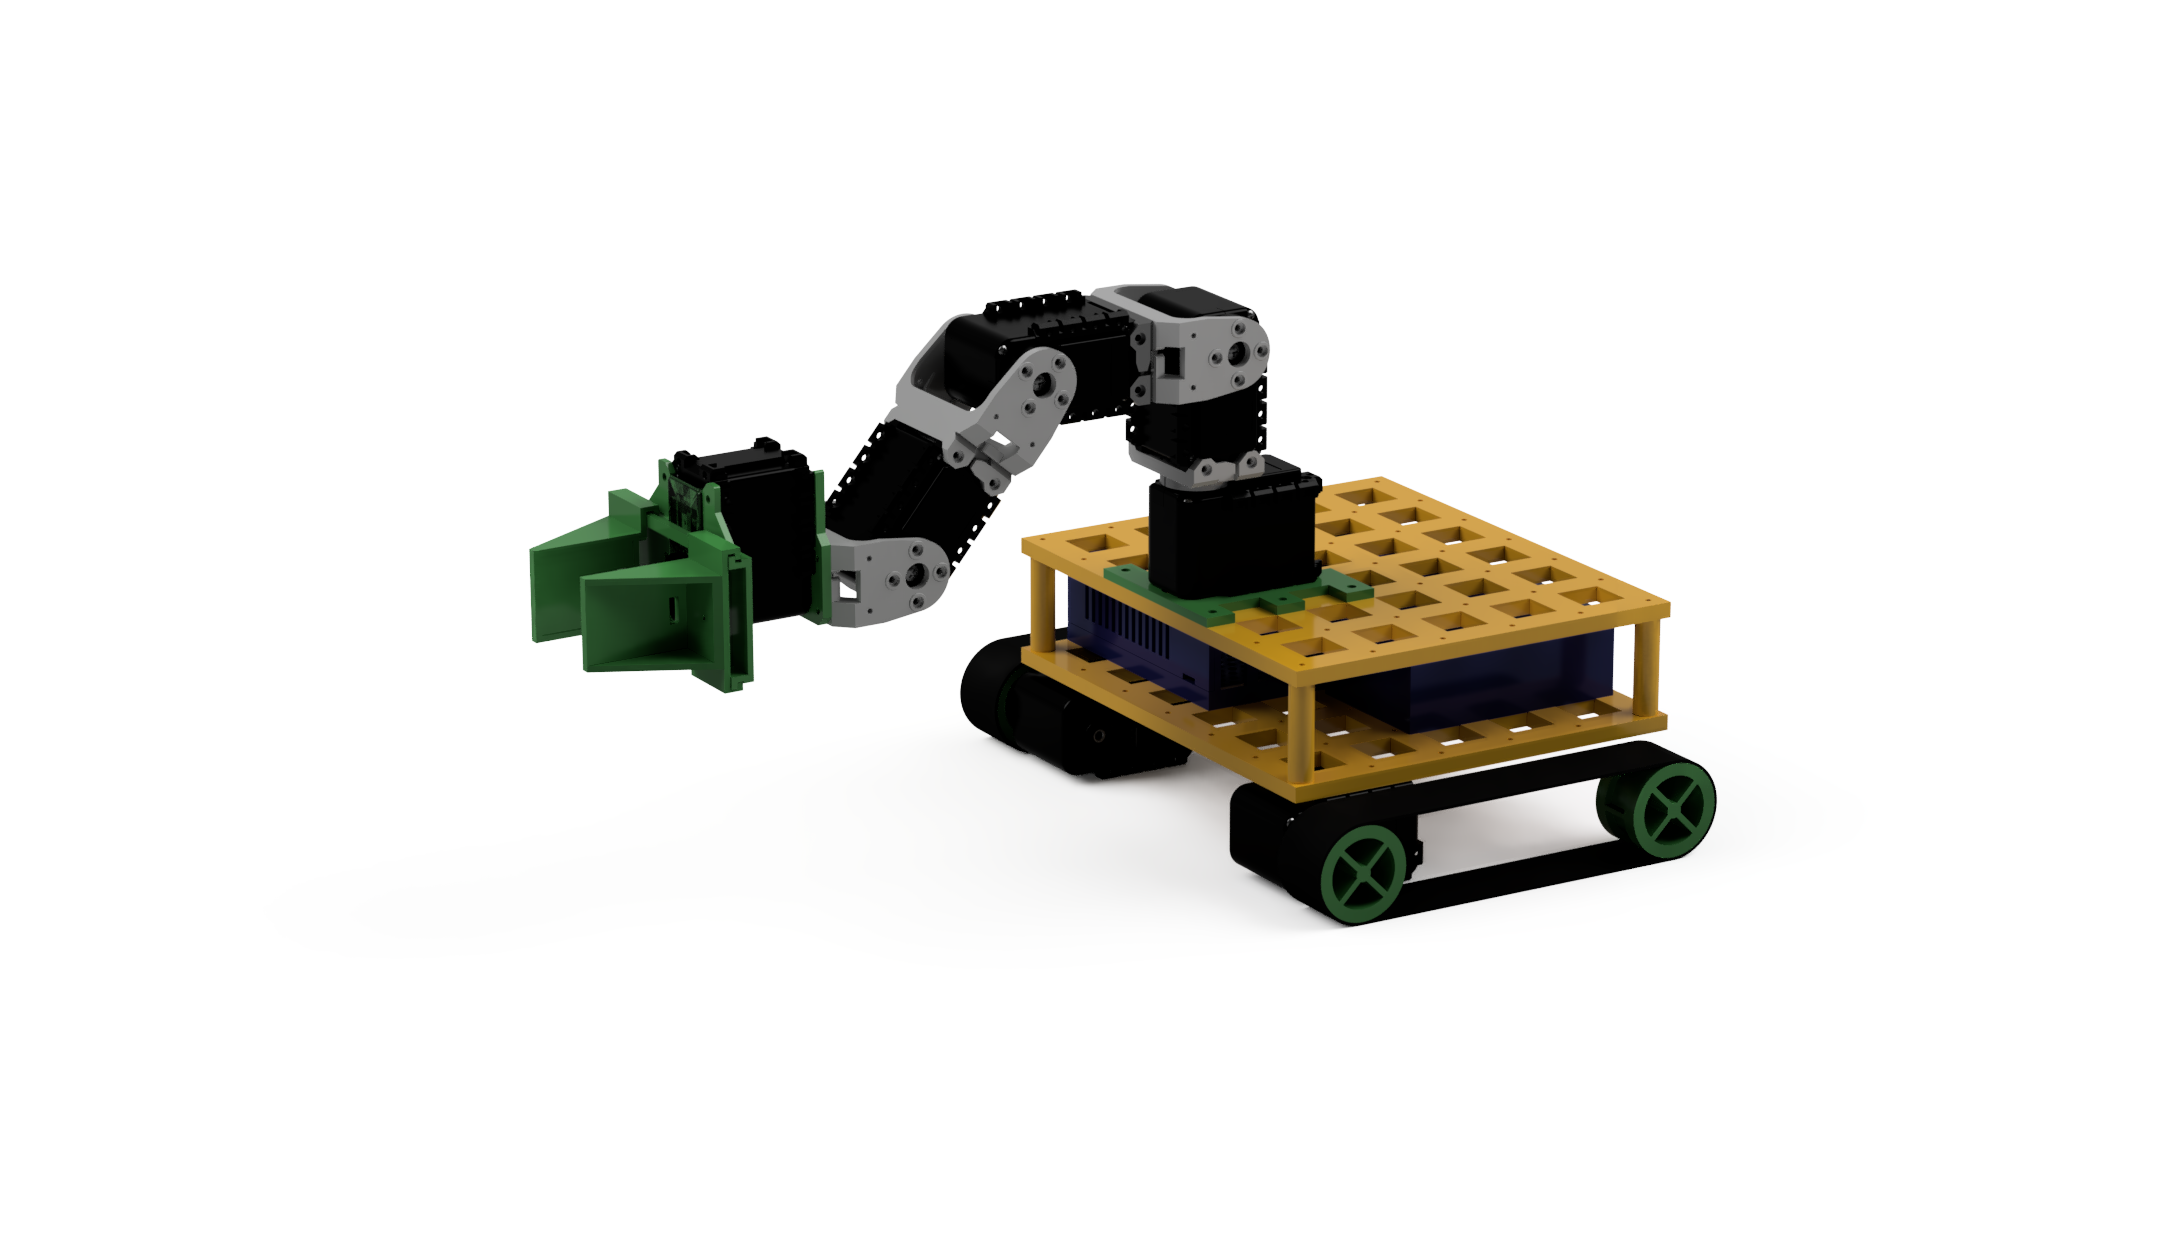
\includegraphics[width=0.7\columnwidth]{chapters/img/rendering.png}
    \caption{Rendering of concept design.}
    \label{fig:concept_rendering}
\end{figure}

\subsection{Electrical components}
While the mechanical components are those visible it's the underlying electrical components that make the big difference. The internals in the Dynamixel\textregistered AX-12A Smart Servo motors give feedback on the state of the motors, the 1000mAh LiPo battery supplies power to the motors and surrounding electronics. For the computations the NVIDIA\textregistered Jetson Nano is used as it runs Ubuntu natively which makes the implementation of the underlying Robotic Operating System (ROS) \cite{ros} faster. 
%\usetikzlibrary{shapes.geometric,arrows, positioning, fit}
\tikzstyle{computing} = [draw, rectangle, fill=white!50, rounded corners, node distance=3em, minimum height=3em]

\tikzstyle{io} = [rectangle, draw, trapezium right angle=110, rounded corners,
                  fill=red!20, node distance=5em, minimum height=2.9em]

\tikzstyle{calculate} = [diamond, draw, trapezium right angle=110, rounded corners,
                  fill=green!20, node distance=1.9cm, minimum height=2.9em]

\tikzstyle{hardware} = [rectangle, draw, trapezium right angle=110, rounded corners,
                  fill=blue!20, node distance=1.9cm, minimum height=2.9em]

\tikzstyle{external} = [rectangle, draw, trapezium right angle=110, rounded corners,
                  fill=gray!20, node distance=1.9cm, minimum height=2.9em]
\tikzstyle{line} = [draw, -latex']

\tikzstyle{function} = [rectangle, draw, fill=green!20, node distance=1.9cm, minimum height=2.9em]

    
    \begin{figure}
        \begin{center}
\resizebox{6.0cm}{!}{

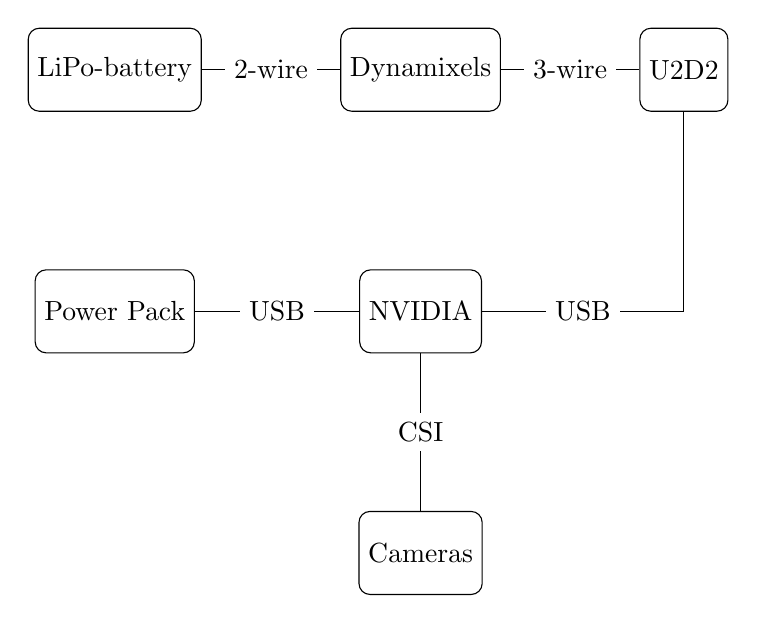
\begin{tikzpicture}

    [align=center, auto]

        \node [computing] (lipo) {LiPo-battery};
        \node [computing, below= of lipo] (powerbank) {Power Pack};
        \node [computing, right= 5em of lipo] (motors) {Dynamixels};
        \node [computing, below= of motors] (nvidia) {NVIDIA};
        \coordinate [below= 1em of motors] (aux1);
        \coordinate [right= of aux1] (aux2);
        \node [computing, right= 5em of motors] (u2d2) {U2D2};
        \node [computing, below= of nvidia] (cameras) {Cameras};
        %\path [line] (nvidia)--(camera);

        \draw [-] (powerbank) -- node[midway, fill=white] {USB} (nvidia);
        \draw [-] (lipo) -- node[midway, fill=white] {2-wire} (motors);
        \draw [-] (motors) -- node[pos=0.5, fill=white] {3-wire} (u2d2);
        \draw [-] (nvidia) -| node[pos=0.25, fill=white] {USB} (u2d2);
        \draw [-] (nvidia) -- node[pos=0.5, fill=white] {CSI} (cameras);
    \end{tikzpicture}
    }
\end{center}
\caption{Diagram of electrical components}
\end{figure}


    %tikz/electrical_connections.tex

\subsection{Robotic Operating System}
Because the robot and the task consists of many different parts it is preferred to utilize an easy to use and well documented framework for internal communication on the robot. With its versatility and popularity within the research community this project makes use of the Robotic Operating System (ROS) as its underlying framework. 
ROS utilizes an internal TCP communication protocol where different parts can communicate and be synchronized which enables real-time performance. 
The rosgraph is shown in Fig. \ref{fig:rosgraph}. 

\begin{figure}
    \centering
    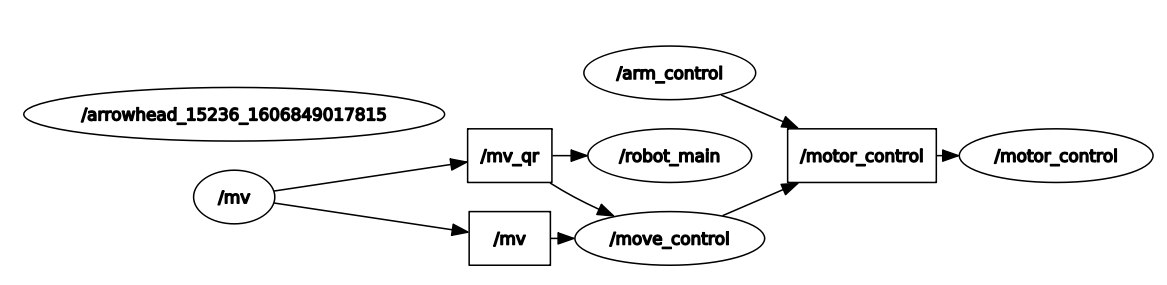
\includegraphics[width=0.7\columnwidth]{chapters/img/rosgraph.jpg}
    \caption{Rosgraph of the robot.}
    \label{fig:rosgraph}
\end{figure}





\subsection{Internals}
\begin{frame}
    \frametitle{NVIDIA Jetson Nano}
    \begin{columns}
        \begin{column}[]{0.5\textwidth}
            \begin{itemize}
                \item Runs Ubuntu
                \item Two camera ports (CSI)
                \item More powerful GPU than RPi
            \end{itemize}
        \end{column}

        \begin{column}[]{0.5\textwidth}
            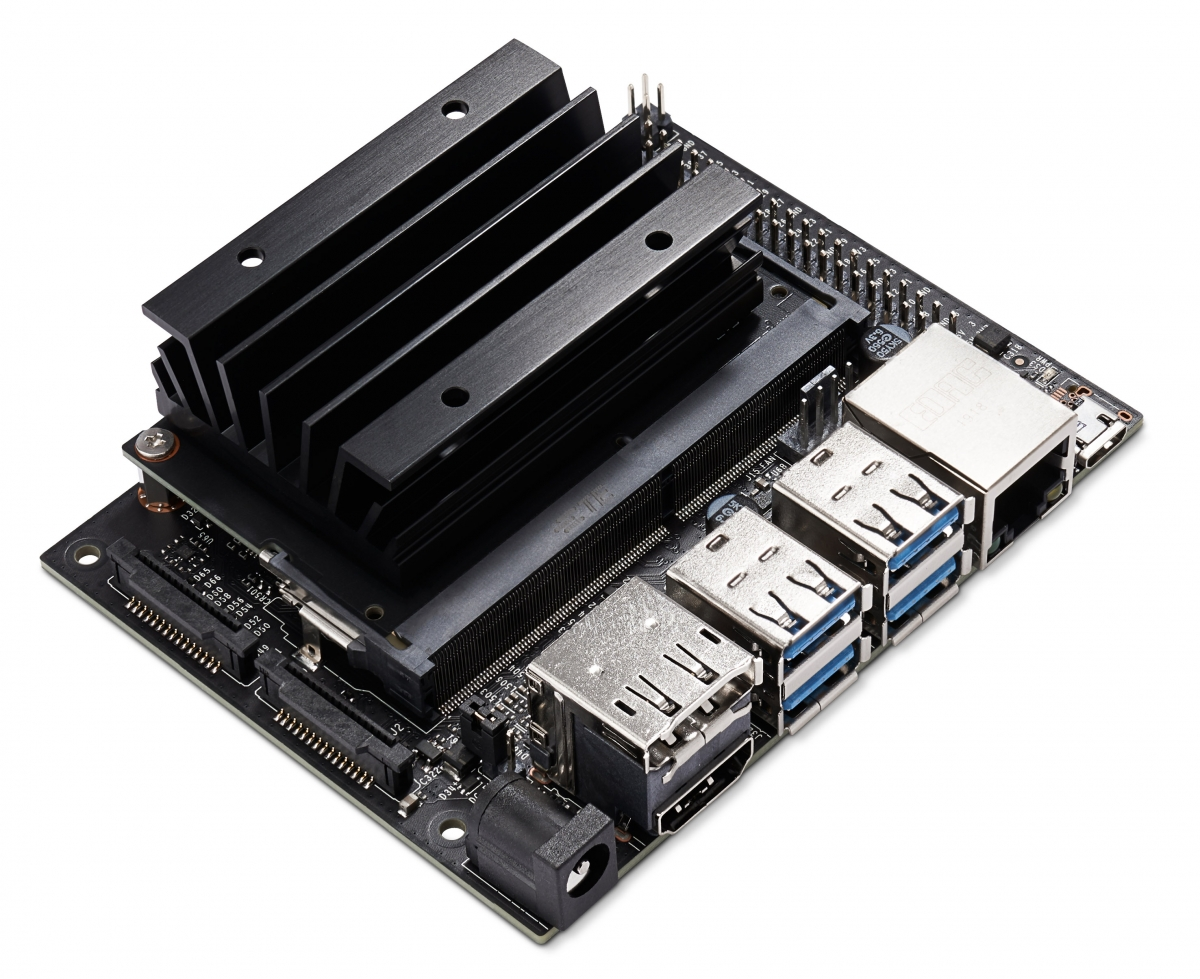
\includegraphics[width=\textwidth]{frames/img/nvidia.jpg}
        \end{column}
    \end{columns}


\end{frame}

\begin{frame}
    \frametitle{Cameras}
    \begin{columns}
        \begin{column}[]{0.5\textwidth}
            \begin{itemize}
                \item Compatible with NVIDIA and RPi
                \item Small package
                \item 8 megapixels
                \item Video:
                \begin{itemize}
                    \item 1080p @ 30 fps
                    \item 720p @ 60fps
                \end{itemize}

            \end{itemize}
        \end{column}

        \begin{column}[]{0.5\textwidth}
            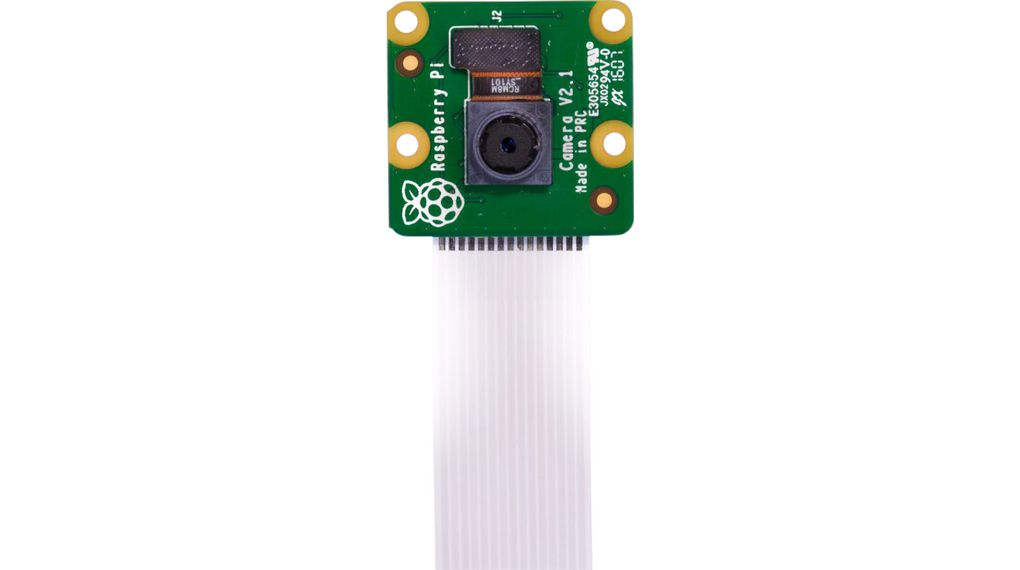
\includegraphics[width=\textwidth]{frames/img/camera.jpg}
        \end{column}
    \end{columns}
\end{frame}


\begin{frame}
    \frametitle{Dynamixel Smart Motors}
    \begin{columns}
        \begin{column}[]{0.5\textwidth}
            \begin{itemize}
                \item Connects in series
                \item Angle and wheel mode
                \item Feedback
            \end{itemize}
        \end{column}

        \begin{column}[]{0.5\textwidth}
            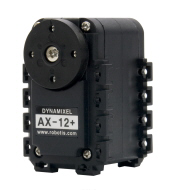
\includegraphics[width=\textwidth]{frames/img/dynamixel.png}
        \end{column}
    \end{columns}
\end{frame}

\begin{frame}
    \frametitle{Hardware}
    \centering
    \resizebox{7.0cm}{!}{
    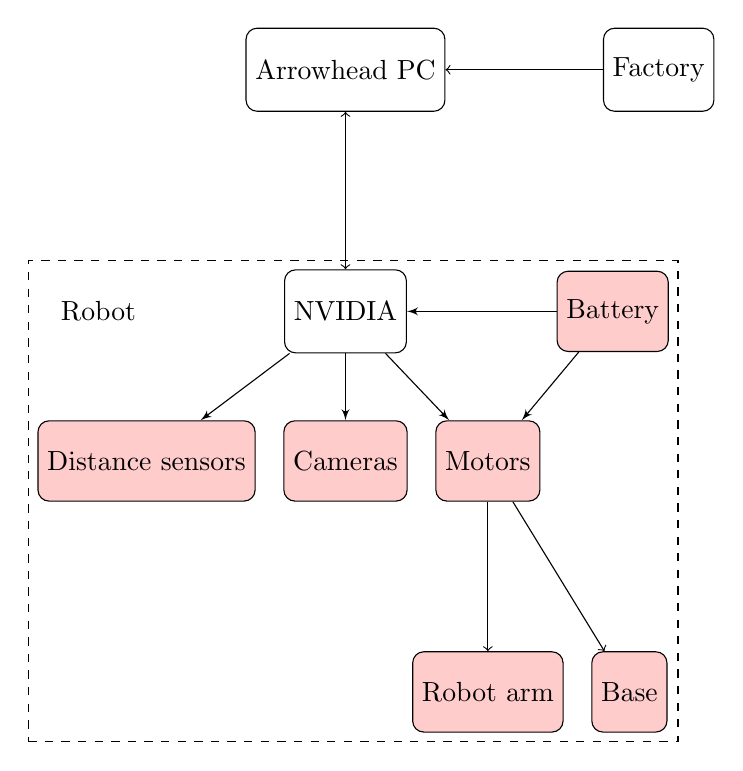
\begin{tikzpicture}
        [align=center, node distance=1em, auto]

        \node [computing] (pc) {Arrowhead PC};
        \node [computing, below= of pc] (nvidia) {NVIDIA};
        \node [io, right= of nvidia] (battery) {Battery};
        \node [computing, right= of pc] (factory) {Factory};
        \node [io, below of= nvidia] (cameras) {Cameras};
        \node [io, right= 1em of cameras] (motors) {Motors};
        \node [io, left= 1em of cameras] (distance_sensors) {Distance sensors};
        \node [io, below= of motors] (arm) {Robot arm};
        \node [io, right= 1em of arm] (base) {Base};
        \node [rectangle=white, left= 5em of nvidia] (robot) {Robot};

        \path [line] (nvidia)--(cameras);
        \path [line] (battery)--(nvidia);
        \path [line] (battery)--(motors);
        \path [line] (nvidia)--(motors);
        \path [line] (nvidia)--(distance_sensors);
        \draw[->] (factory) -- (pc);
        \draw[<->] (pc) -- (nvidia);
        \draw[->] (motors) -- (arm);
        \draw[->] (motors) -- (base);
        \node [draw=black, dashed, fit= (nvidia) (battery) (distance_sensors)
        (cameras) (motors) (base) (arm)]{};

    \end{tikzpicture}
    }
\end{frame}


\begin{frame}
    \frametitle{Concept rendering}
    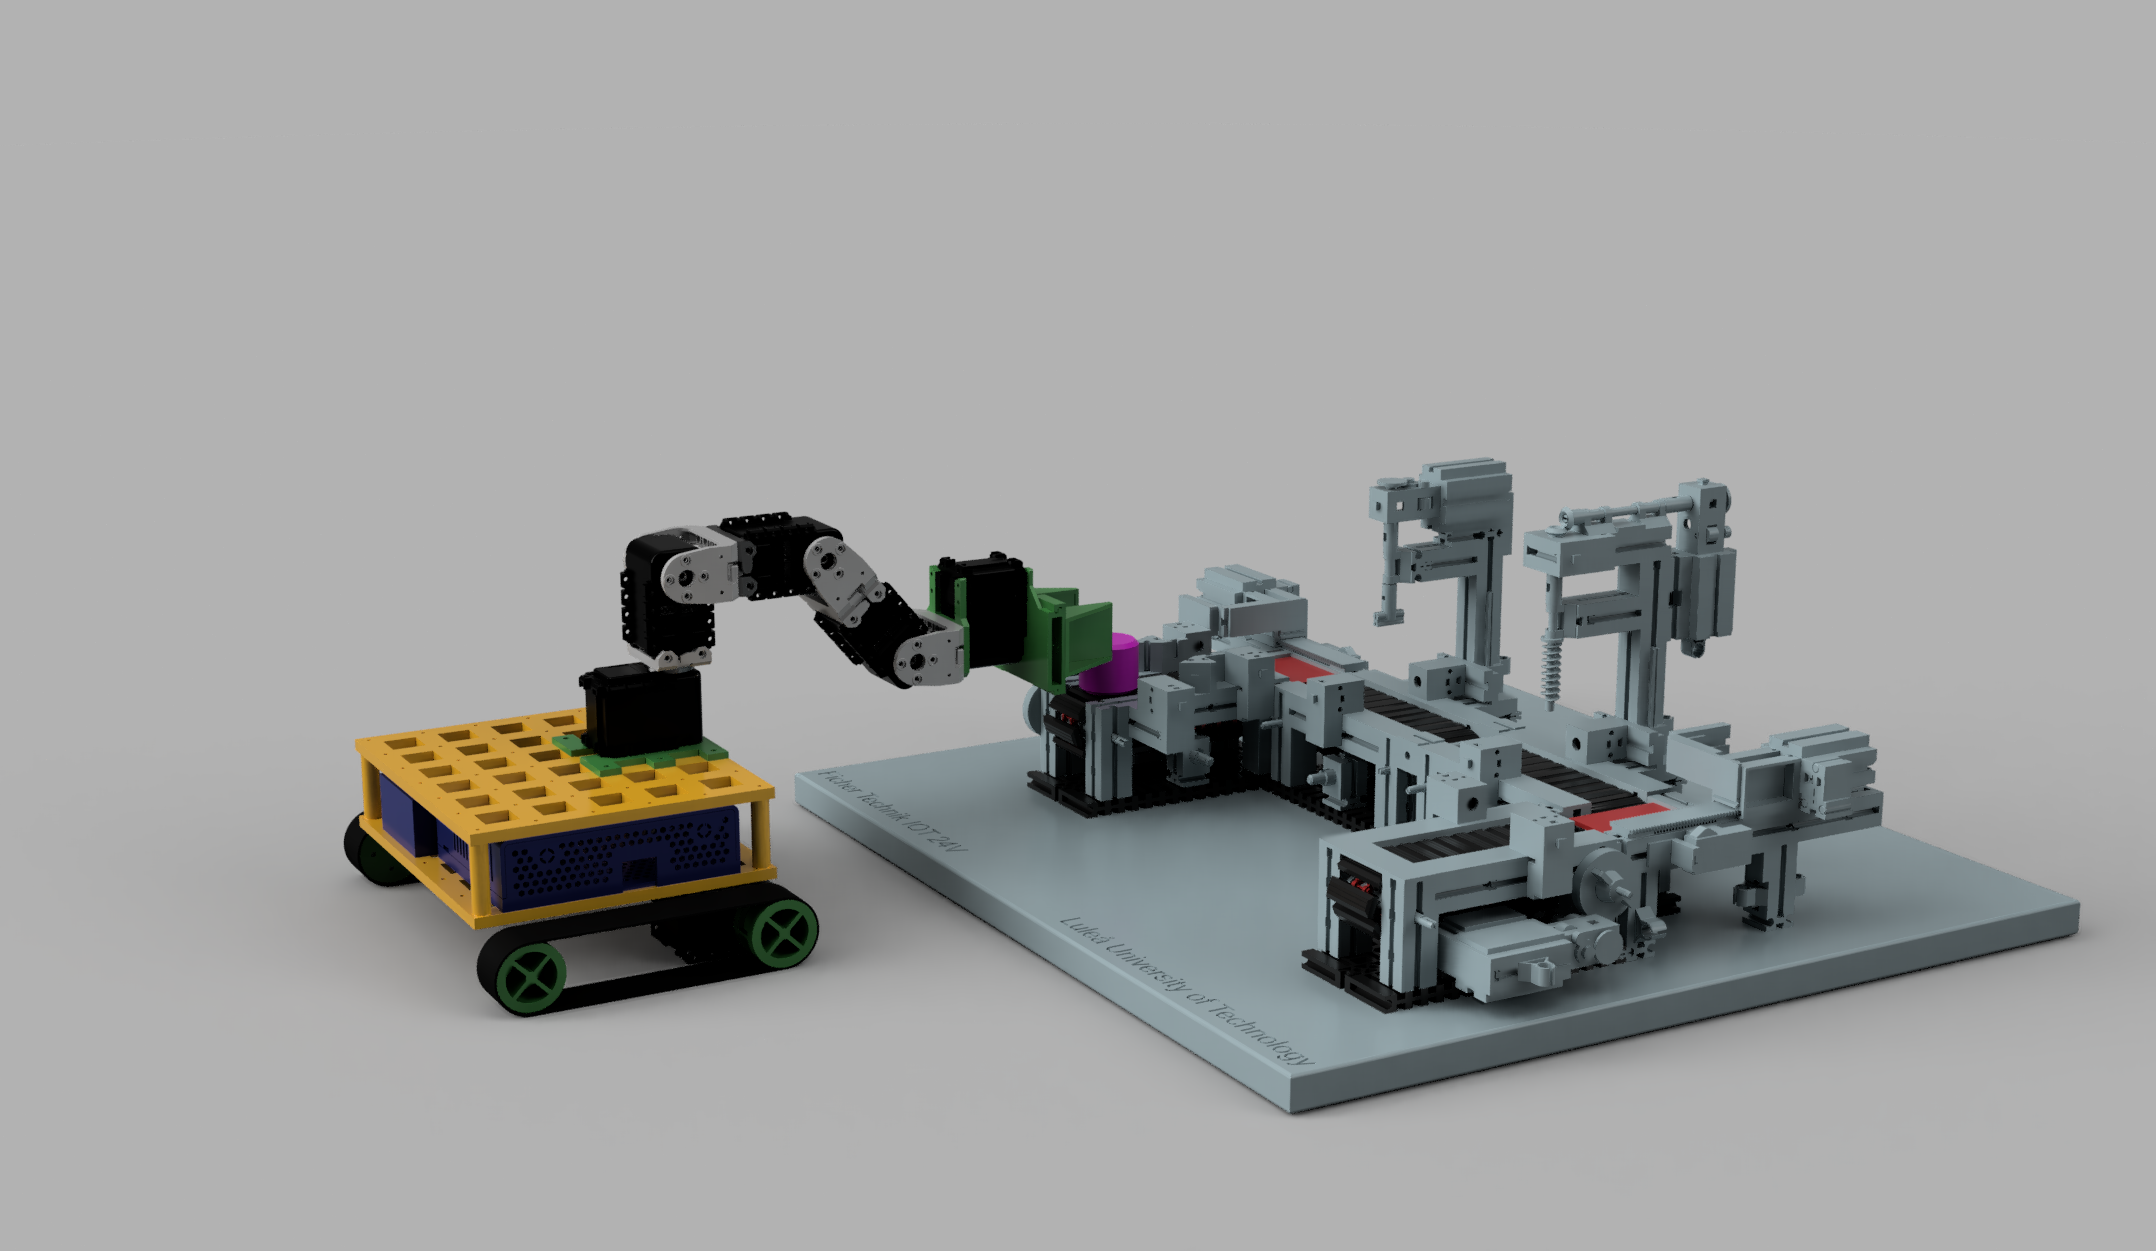
\includegraphics[width=\textwidth]{frames/img/b4_manufacturing.PNG}
\end{frame}
\subsection{Flowcharts}

\resizebox{9.0cm}{!}{

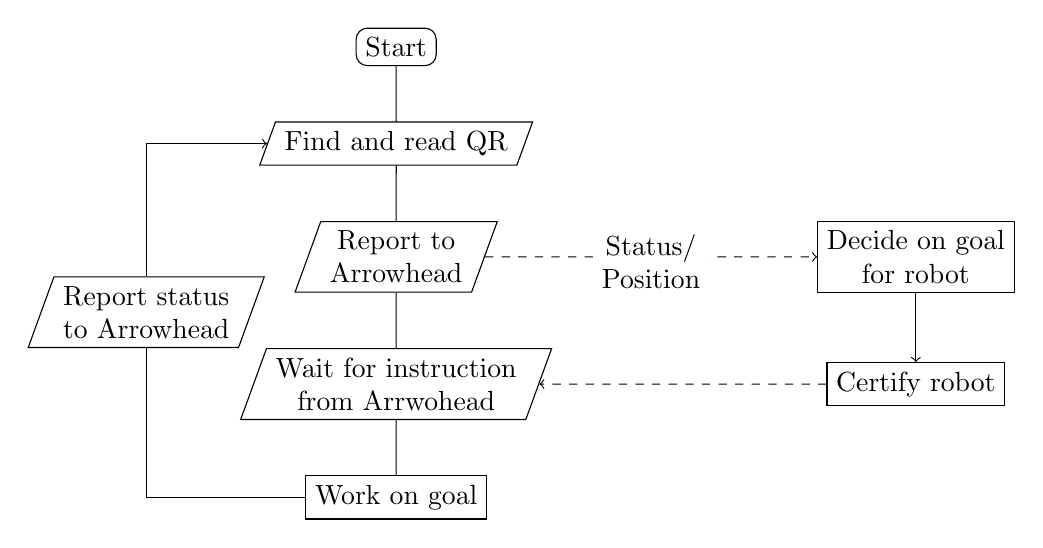
\begin{tikzpicture}
    [align=center, node distance = 2em,  auto]

    %% Robot
    \node [Start] (start) {Start};
    \node [Data, below= of start] (findqr) {Find and read QR};
    \node [Data, below= of findqr] (report) {Report to \\ Arrowhead};
    \node [Data, below= of report] (getgood) {Wait for instruction \\from Arrwohead};
    \node [Process, below= of getgood] (follow) {Work on goal};
    \node [Data, left= of report, yshift=-2em] (status) {Report status \\ to Arrowhead};

    %% Arrowhead
    \node [Process, right= of report, xshift=10em] (arrowstart) {Decide on goal \\ for robot};
    \node [Process, below= of arrowstart, yshift=-0.5em] (certify) {Certify robot};


    %% Draw
    \draw (start) -- (findqr) -- (report) -- (getgood) -- (follow);
    \draw [->] (follow) -| (status) |- (findqr);

    
    \draw [->, dashed] (report) -- node[midway, fill=white, yshift=-1.5em] {Status/ \\ Position} (arrowstart);
    \draw [->] (arrowstart) -- (certify);
    \draw [->, dashed] (certify) -- (getgood);

\end{tikzpicture}
}
\begin{frame}
    \frametitle{ROS-Base example}
\begin{center}
    

    \resizebox{8.0cm}{!}{
    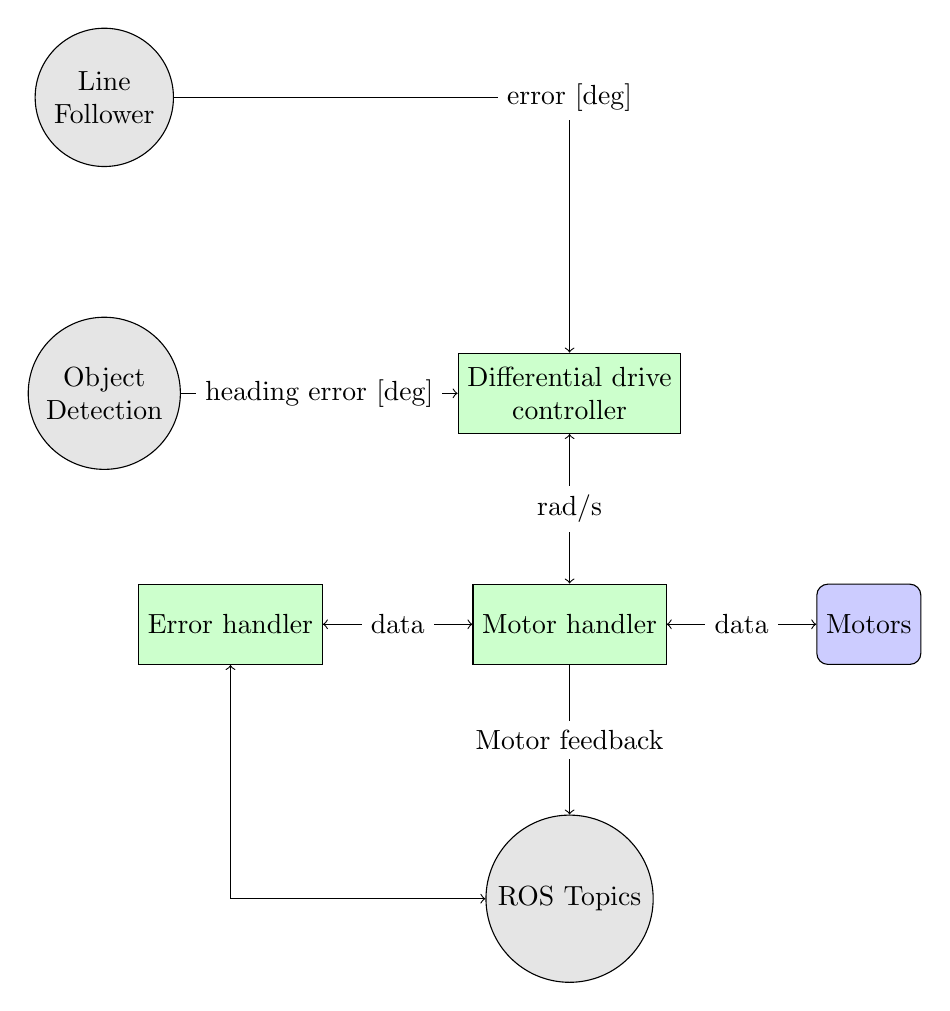
\begin{tikzpicture}
        [align=center]
        \node [ros] (line) {Line \\Follower};
        \coordinate [below= of line] (aux1);
        \node [ros, below= of line] (obj) {Object\\ Detection};
        \node [function, right= 10em of obj] (diff) {Differential drive\\controller};
        \node [function, below= of diff] (handler) {Motor handler};
        \node [function, left= of handler] (error) {Error handler};
        \node [hardware, right= of handler] (motors) {Motors};
        \node [ros, below= of handler] (ros) {ROS Topics};
    
        
        
    
        \draw [->] (line) -| node[midway, fill=white] {error [deg]} (diff);
        \draw [<->] (diff) -- node[midway, fill=white] {rad/s} (handler);
        \draw [<->] (handler) -- node[midway, fill=white] {data} (motors);
        \draw [->] (handler) -- node[midway, fill=white] {Motor feedback} (ros);
        \draw [->] (obj) -- node[midway, fill=white] {heading error [deg]} (diff);
        \draw [<->] (error) -- node[midway, fill=white] {data} (handler);
        \draw [<->] (error) |- (ros);
        
    \end{tikzpicture}
    }
\end{center}
\end{frame}
\input{frames/factory.tex}

\section{Machine Vision}
\subsection{EDWARD USE SUBSECTIONS!}
\begin{frame}
    \begin{center}
        \Huge Machine vision
    \end{center}
\end{frame}





%%%%%%%%%%%% Add new frames above this line %%%%%%%%%


\begin{frame}
    \begin{center}
        \Huge Questions?
    \end{center}
\end{frame}





\end{document}